\documentclass[aspectratio=169,usenames,dvipsnames]{beamer}
\usetheme{Pittsburgh}
\usepackage{xcolor}
\usepackage[utf8]{inputenc}
\usepackage[german]{babel}
\usepackage{amsmath}
\usepackage{amsfonts}
\usepackage{amssymb}
\usepackage{graphicx}
\usepackage{multicol}
\usepackage{wrapfig}
\usepackage{hyperref}
\usepackage{pdfrender}

\author{Jonas Betzendahl}
\title{Papageien am Steuer}

\beamertemplatenavigationsymbolsempty 

%src: https://tex.stackexchange.com/questions/34921/how-to-overlap-images-in-a-beamer-slide
\def\Put(#1,#2)#3{\leavevmode\makebox(0,0){\put(#1,#2){#3}}}

\definecolor{TitleColour}{rgb}{1,1,0}
\definecolor{lightestgray}{rgb}{0.95,0.95,0.95}

\begin{document}
\sffamily

%------------------------------------------------------------------------------------
\section{Introduction}

{
    \usebackgroundtemplate{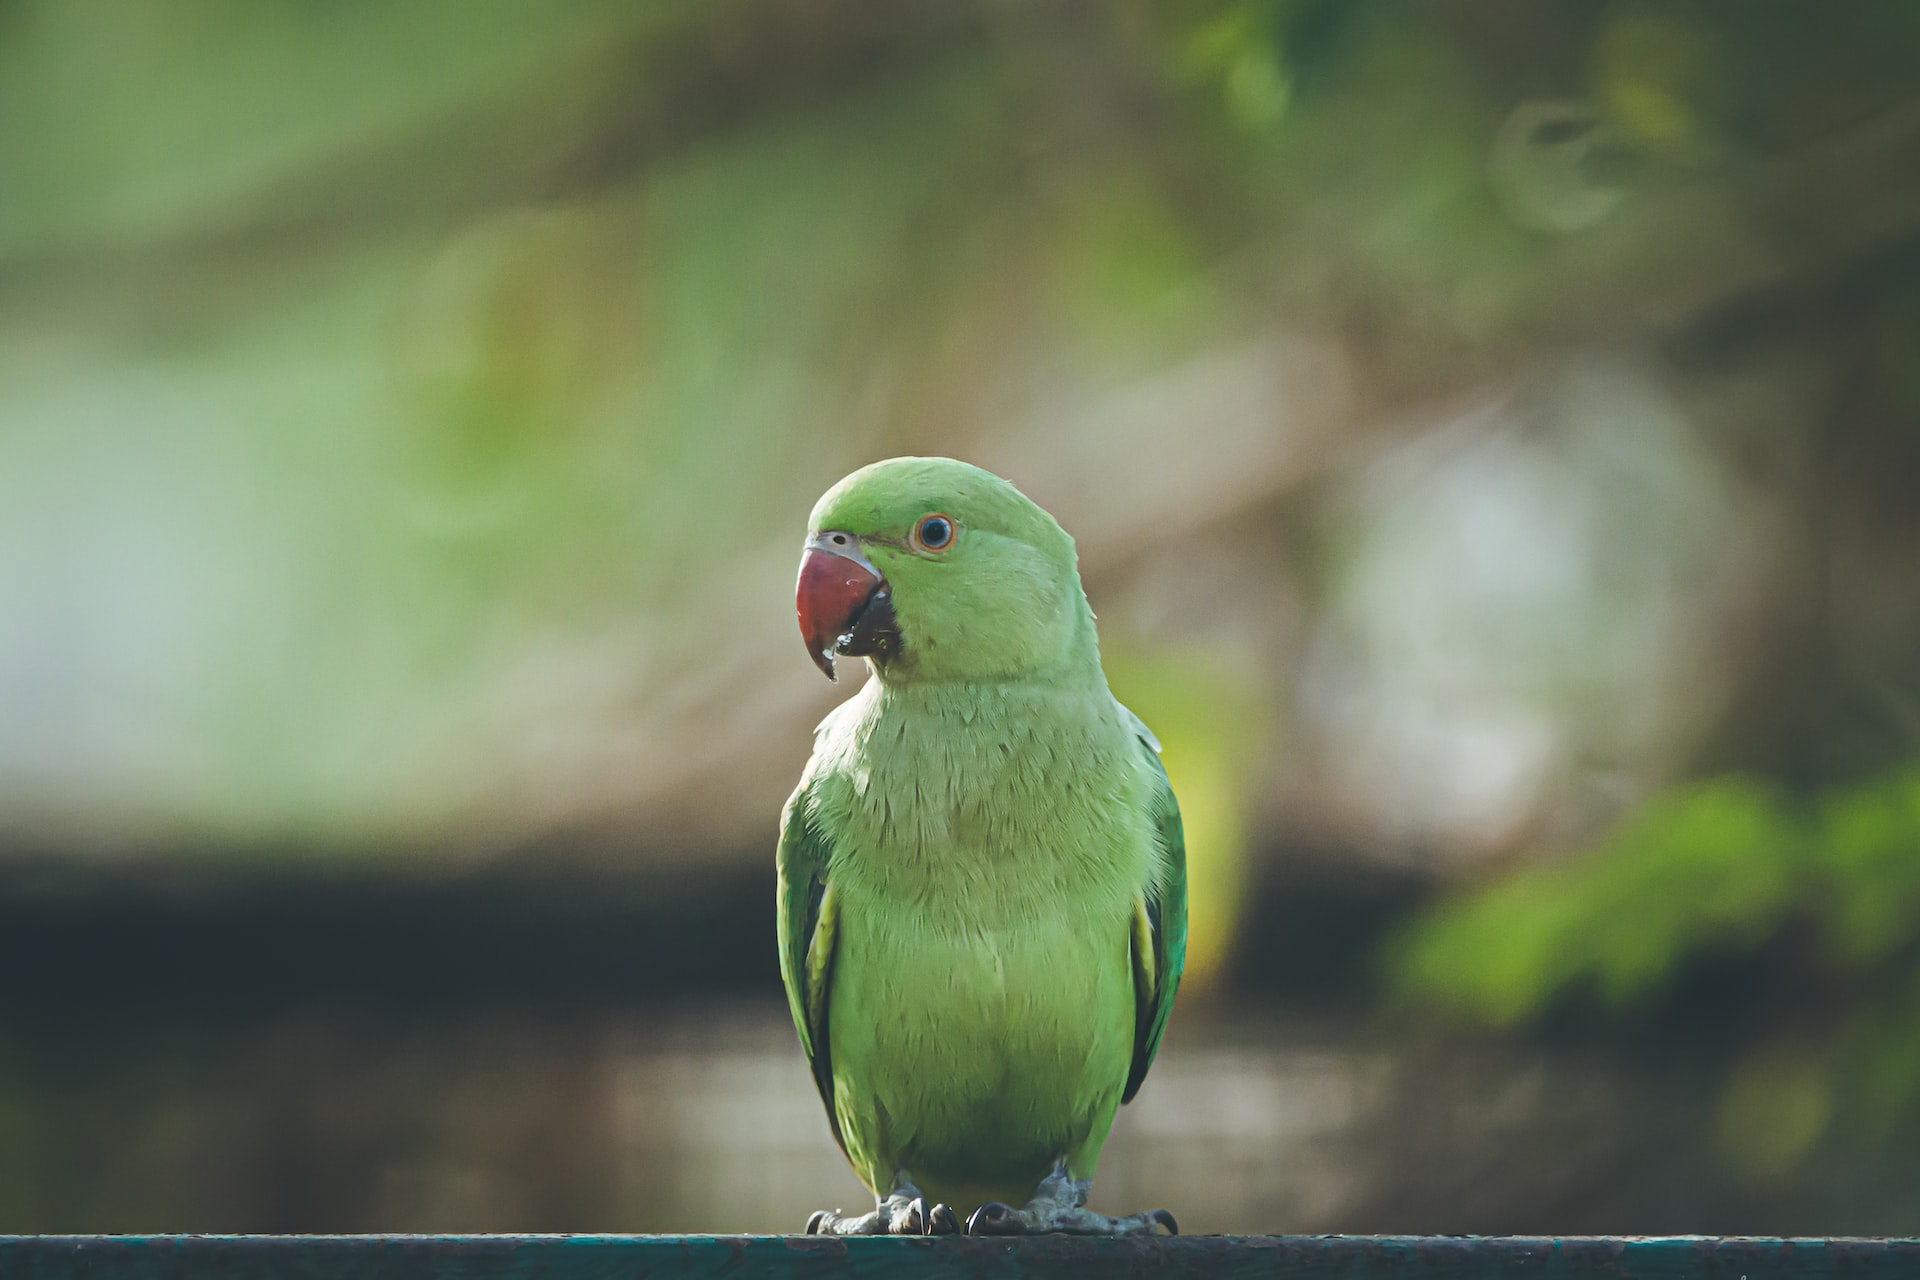
\includegraphics[height=\paperheight,width=\paperwidth]{images/parrot_titlecard}}
    \setbeamertemplate{navigation symbols}{}
    \begin{frame}[fragile]
    \Put(-20,160){\textpdfrender{
		TextRenderingMode=FillStroke,
		LineWidth=.2pt,
		FillColor=TitleColour,
	}{\resizebox{0.75\linewidth}{!}{Papageien am Steuer!}}
    }
    
    \Put(-20,130){\textpdfrender{
		TextRenderingMode=FillStroke,
		LineWidth=.1pt,
		FillColor=TitleColour,
	}{\resizebox{0.85\linewidth}{!}{ChatGPT und die Zukunft von Künstlicher Intelligenz}}
    }
    
    \Put(-20,100){
        \large
	\textcolor{yellow}{Jonas Betzendahl, M.Sc.}
    }
    \Put(-23,70){
	\textcolor{yellow}{FAU Erlangen - Nürnberg}
    }
    \Put(300,-180){
	\href{https://github.com/lambdaTotoro}{
\includegraphics[scale=0.125]{images/github_logo.png}}
	\href{https://chaos.social/@lambdatotoro}{\includegraphics[scale=0.125]{images/mastodon_logo.png}}
	\href{https://twitter.com/lambdatotoro}{
\includegraphics[scale=0.125]{images/twitter_logo.png}}
    }
    \Put(230,-220){
	\textcolor{white}{\texttt{@LambdaTotoro (@chaos.social)}}
    }
    \end{frame}
}

\setbeamercolor{background canvas}{bg=lightestgray}

%------------------------------------------------------------------------------------

\begin{frame}
\begin{center}
\Large
Teil I:
\bigskip

\huge
\emph{Tschätt Jeepy Wer\dots?}
\end{center}
\end{frame}

\begin{frame}
\begin{minipage}{0.45\textwidth}
\vfill
$$\qquad$$
\vfill
\end{minipage}%
\begin{minipage}{0.55\textwidth}
\vfill
\begin{itemize}
\item ChatBot-Modell: Text rein $\rightarrow$ Text raus
\item Buzzwords:\\
Transformer-based Large Language Model
\item Trainiert auf großen Teilen des Internets:
\end{itemize}
\end{minipage}
\Put(0, 25){
\includegraphics[width=0.4\textwidth, keepaspectratio]{images/OpenAI_Logo}}
\pause
\Put(210, -30){$\cdot$ Wikipedia,}
\pause
\Put(206, -60){$\cdot$ Internet Archive,}
\pause
\Put(202, -90){$\cdot$ Social Media (Twitter, Reddit, \dots),}
\Put(199, -120){$\cdot$ Nachrichtenseiten,}
\Put(195, -150){$\cdot$ Wissenschaftliche Papiere,}
\Put(191, -180){$\cdot$ Common Crawl Corpus,}
\Put(187, -210){$\cdot$ BooksCorpus,}
\Put(183, -240){$\cdot$ Project Gutenberg,}
\pause
\Put(-50, -240){
\includegraphics[width=0.5\linewidth, keepaspectratio]{images/elon_torso} }
\end{frame}

%------------------------------------------------------------------------------------

\begin{frame}
\frametitle{Beispiel}
\end{frame}

\begin{frame}
\frametitle{ChatFAQ}
\end{frame}

\begin{frame}
\frametitle{Wie funktioniert ChatGPT?}
\end{frame}

\begin{frame}
\frametitle{Profiteure und Potential}
\end{frame}

\begin{frame}
\begin{center}
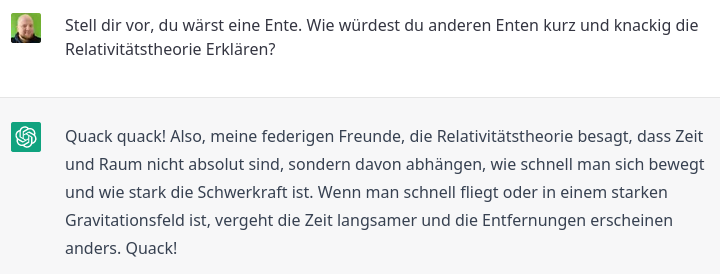
\includegraphics[width=0.9\linewidth, keepaspectratio]{images/conversation_01} 
\end{center}
\pause
\Put(300,-125){
\includegraphics[width=0.3\linewidth, keepaspectratio]{images/happy_rubber_duck}}
\end{frame}

\section{Trouble in Paradise}
\begin{frame}
\begin{center}
\Large
Teil II:
\bigskip

\huge
\emph{Ärger im Paradies}
\end{center}
\end{frame}

\begin{frame}
\begin{center}
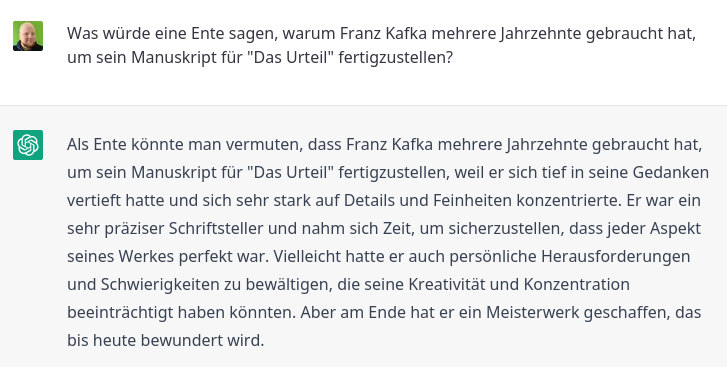
\includegraphics[width=0.9\linewidth, keepaspectratio]{images/conversation_02} 
\end{center}
\pause
\Put(350,-125){
\includegraphics[width=0.3\linewidth, keepaspectratio]{images/angry_duckling}}
\end{frame}

%------------------------------------------------------------------------------------

\begin{frame}
\frametitle{Wie funktioniert ChatGPT wirklich?}
\end{frame}

{
    \usebackgroundtemplate{
\includegraphics[height=\paperheight,width=\paperwidth]{images/wbw_card}}
    \setbeamertemplate{navigation symbols}{}
    \begin{frame}[fragile]
    \Put(50,-70){\textpdfrender{
		TextRenderingMode=FillStroke,
		LineWidth=.2pt,
		FillColor=TitleColour,
	}{\resizebox{0.4\linewidth}{!}{Lust auf mehr?}}
    }
    
    \Put(-5,-95){\textpdfrender{
		TextRenderingMode=FillStroke,
		LineWidth=.1pt,
		FillColor=white,
		StrokeColor=white,
	}{\resizebox{0.6\linewidth}{!}{12 slammige Beiträge zu KI, Klima, Gender\dots}}
    }
    
    \Put(15,-115){\textpdfrender{
		TextRenderingMode=FillStroke,
		LineWidth=.1pt,
		FillColor=white,
		StrokeColor=white,
	}{\resizebox{0.3\linewidth}{!}{Extra viel Wissenschaft!}}
    }
    \Put(-15,-145){\textpdfrender{
		TextRenderingMode=FillStroke,
		LineWidth=.1pt,
		FillColor=white,
		StrokeColor=white,
	}{\resizebox{0.65\linewidth}{!}{Das perfekte Geschenk für konservative Nervensägen!}}
    }
    
    \Put(-5,-165){\textpdfrender{
		TextRenderingMode=FillStroke,
		LineWidth=.1pt,
		FillColor=white,
		StrokeColor=white,
	}{\resizebox{0.55\linewidth}{!}{Verfügbar online, im Buchhandel und bei mir!}}
    }
    \end{frame} 
}

\begin{frame}
\frametitle{Wie funktioniert ChatGPT wirklich? (Publikum)}
\end{frame}

\begin{frame}
\frametitle{The Semantics Problem}
\end{frame}

\begin{frame}
\frametitle{Stochastic Parrots}
\end{frame}

\begin{frame}
\begin{center}
\Large
Teil III:
\bigskip

\huge
\emph{Papageien gegen Affen}
\end{center}
\end{frame}

\begin{frame}
\frametitle{Reinforcing Human Biases}
\end{frame}

\begin{frame}
\frametitle{Kenia Exploitation}
\end{frame}

\begin{frame}
\frametitle{Not as invincible as you thought}
\end{frame}

%------------------------------------------------------------------------------------

\section{Werbung \& Ende}

\begin{frame}
\frametitle{Take-Home Messages}
\end{frame}

\begin{frame}[fragile]
\frametitle{Quellen:}
\scriptsize
\begin{center}
``Weltrettung braucht Wissenschaft''

\url{www.amazon.de/Weltrettung-braucht-Wissenschaft-Antworten-dr%C3%A4ngenden/dp/3499010062}
\end{center}
\medskip

\begin{itemize}
\item Try it yourself: \url{https://chat.openai.com}
\item Bender, Gebru et al.: ``On the Dangers of Stochastic Parrots: Can Language Models Be Too Big?'' \url{https://dl.acm.org/doi/pdf/10.1145/3442188.3445922}
\item 11KM-Podcast (tagesschau): ``Schafft ChatGPT das Abi? (das bayerische!)'' \url{https://www.ardaudiothek.de/episode/11km-der-tagesschau-podcast/schafft-chatgpt-das-abi-das-bayerische/tagesschau/12396019/}
\item TIME: ``OpenAI Used Kenyan Workers on Less Than $\$$2 Per Hour to Make ChatGPT Less Toxic'': \url{https://time.com/6247678/openai-chatgpt-kenya-workers/}
\end{itemize}
\end{frame}
\end{document}

